\section{FKM Richtlinien}{}
    \subsection{Auslastungsgrad}
     
        \subsubsection{Definitionen}
            \begin{enumerate}[noitemsep]
                \item $\sigma_{v}$: Vergleichsspannung im Nachweispunkt
                \item $\sigma_{SK}$: Materialfestgkeit, bauteilspezifisch
                \item $J_{ges}$: Sicherheitsfaktor (Gesamtsicherheitsfaktor)
            \end{enumerate}
            \[a_{SK} = \frac{\sigma_{v}}{\sigma_{sk}/J_{ges}} \]
    
        \subsubsection{Mehrachsigkeit}
            Falls $h > 1.33$ zusätzlicher Nachweis erforderlich! 
            \[ h = \frac{\frac{1}{3} \textrm{Spur}[T]}{\sigma_{Mises}} \quad \textrm{[T]: Spannungstensor}\]
        \subsubsection{Bauteilfestigkeit $\sigma_{\textrm{SK}}$}
            An Normprobe gemessene Fliessgrenze erffordert meistens Korrektur! \\$R_P$: Fliessgrenze Bauteil; $R_{P,N}$: Fliessgrenze Normporbe.
            \[R_P = K_{d,P}\cdot K_A\cdot R_{P,N}\]
            \[\sigma_{\textrm{SK}}=R_p\cdot n_{\textrm{pl}} \quad\textrm{mit:}\quad \small n_{\textrm{pl}}=\textrm{min} \left( \sqrt{ \frac{E\cdot\varepsilon_{\textrm{ertr}}}{R_p}};K_p \right) \]\normalsize
            Hom. Spannungsverteilung: $N_{\textrm{pl}}=1$ (Keine Reserve)
            \[K_p: \textrm{platische Formzahl} = \frac{\textrm{vollplastische Traglast}}{\textrm{elastische Grenzlast}}\]
            vollpl.: aus FE, el. Grenzl.: wenn $\sigma_v$ $R_p$ erreicht.
        \subsubsection{Sicherheitsfaktor $J_{\textrm{ges}}$}
        \small\[J_{\textrm{ges}}= J_s \cdot \left[ J_z \cdot \textrm{max}\left(\frac{J_m \cdot R_p}{R_m}; J_p \right) \right] \]\normalsize
        $J_s$: Lastfaktor (Sicher:=1); $J_z$: Schweissteile; $J_p$: plastifizierung
        \begin{center}
            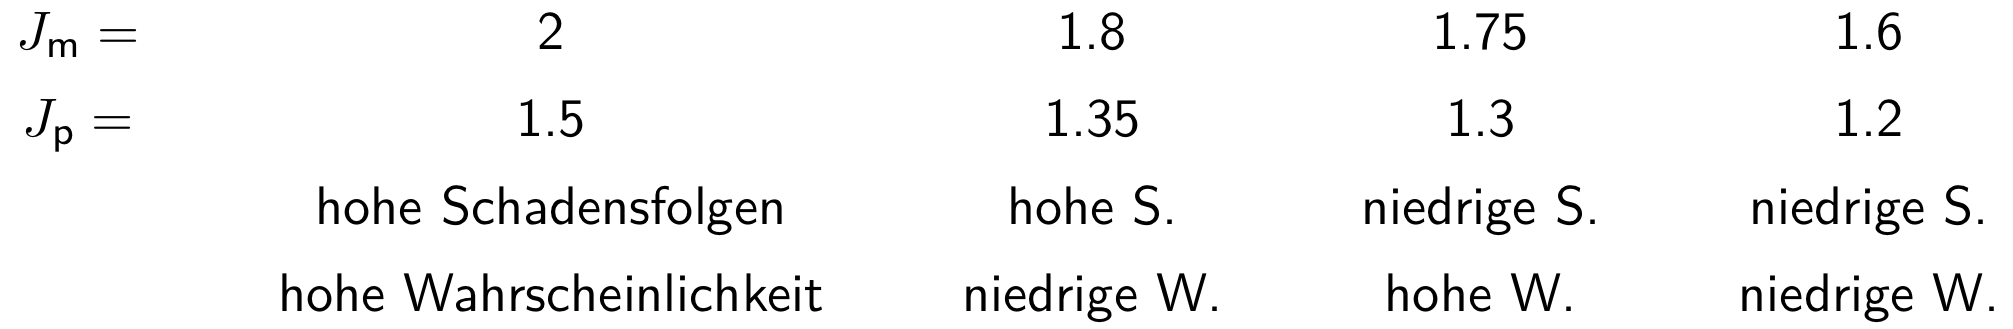
\includegraphics[width=0.8\linewidth]{05/Sicherheitsfaktoren.png}
        \end{center}
    
    \subsection{BSP}
        \TODO{BSP VON SERIE}